% This is the Reed College LaTeX thesis template. Most of the work 
% for the document class was done by Sam Noble (SN), as well as this
% template. Later comments etc. by Ben Salzberg (BTS). Additional
% restructuring and APA support by Jess Youngberg (JY).
% Your comments and suggestions are more than welcome; please email
% them to cus@reed.edu
%
% See http://web.reed.edu/cis/help/latex.html for help. There are a 
% great bunch of help pages there, with notes on
% getting started, bibtex, etc. Go there and read it if you're not
% already familiar with LaTeX.
%
% As far as I know, this follows the requirements laid out in 
% the 2002-2003 Senior Handbook. Ask a librarian to check the 
% document before binding. -SN

%%
%% Preamble
%%
% \documentclass{<something>} must begin each LaTeX document
\documentclass[12pt,twoside]{reedthesis}
% Packages are extensions to the basic LaTeX functions. Whatever you
% want to typeset, there is probably a package out there for it.
% Chemistry (chemtex), screenplays, you name it.
% Check out CTAN to see: http://www.ctan.org/
%%
\usepackage{graphicx,latexsym} 
\usepackage{amssymb,amsthm,amsmath}
\usepackage{longtable,booktabs,setspace} 
\usepackage{chemarr} %% Useful for one reaction arrow, useless if you're not a chem major
\usepackage[hyphens]{url}
\usepackage{rotating}
\usepackage{natbib}
\usepackage[utf8]{inputenc}

% Packages added by Me
%###############################
\usepackage{epigraph}
\usepackage{mathdesign}
\usepackage[hang, flushmargin]{footmisc}
%###############################

% Comment out the natbib line above and uncomment the following two lines to use the new 
% biblatex-chicago style, for Chicago A. Also make some changes at the end where the 
% bibliography is included. 
%\usepackage{biblatex-chicago}
%\bibliography{thesis}

% \usepackage{times} % other fonts are available like times, bookman, charter, palatino

\title{The Effect of Maternal Separation on the Stress Response of
  \textit{A. burtoni}}
\author{Marissa Breanne Borrego}
% The month and year that you submit your FINAL draft TO THE LIBRARY (May or December)
\date{May 2019}
%\division{Mathematics and Natural Sciences}
\advisor{Suzy C. P. Renn}
%If you have two advisors for some reason, you can use the following
%\altadvisor{Your Other Advisor}
%%% Remember to use the correct department!
\department{Neuroscience}
% if you're writing a thesis in an interdisciplinary major,
% uncomment the line below and change the text as appropriate.
% check the Senior Handbook if unsure.
\thedivisionof{The Established Interdisciplinary Committee for Neuroscience}
% if you want the approval page to say "Approved for the Committee",
% uncomment the next line
\approvedforthe{Committee}

\setlength{\parskip}{0pt}
%%
%% End Preamble
%%
%% The fun begins:
\begin{document}

  \maketitle
  \frontmatter % this stuff will be roman-numbered
  \pagestyle{empty} % this removes page numbers from the frontmatter

% Acknowledgements (Acceptable American spelling) are optional
% So are Acknowledgments (proper English spelling)
    \chapter*{Acknowledgements}
	\epigraph{Any situation in which some individuals prevent others from engaging in the process of inquiry is one of violence.}{\textit{Paulo Freire \\ Pedagogy of the Oppressed}}
	
	I have been so very privileged to have the experience of attending college and
  writing a thesis. I would like to thank:\\
	
$\circ$ Suzy for pushing me to take the thesis process into my own hands and not
  giving up on me. Also to the rest of the Renn lab for helping me learn the ways of fish research.

 $\circ$ Paul for mentoring me throughout my undergraduate experience and giving me so many opportunities to learn. 	
  
$\circ$ Larry for supporting me in my research and giving me so much encouragement and
  so many resources. 

 $\circ$ Karen and Jonathan for taking me to libraries, parks, museums, concerts, and the like.
  Not bad for a couple of eloped, new wave-loving kids. 
	
	$\circ$ Presence for
  letting me curl up in a ball on the floor, for
  encouraging me to challenge the systems I am a part of, for so much more.

 $\circ$ Pax, Pixie, and Noah for accompanying me on weird adventures through Eastern
  Oregon and through exploring my identity.
	
$\circ$ James for inspiring me to study neuroscience and for giving me endless love
  and support.

 $\circ$ Matt for being a constant source of positivity and a great listener.

$\circ$ Sonya for keeping up the puke \& rally spirit while working in the library.

 $\circ$ Langston for ensuring that I made it out of this year alive and for supporting my curiosities in math, programming, communicative
  relationships, softness, pretentious Portland stereotypes, etc.

$\circ$ Sarah, Sage, and Cody for never questioning why I was always in your house.

$\circ$ Duncan for opening your arms after every time I ignored your advice and then regretted doing so. You are such a strong being.

 $\circ$ Cam for being a great friend, an absent roommate, an incredible scientist, and perhaps most importantly, a truly interesting person.
	

% The preface is optional
% To remove it, comment it out or delete it.
    \chapter*{Preface}
	Science has a history as an oppressive institution. That being said, I think
  that science also has the ability to liberate individuals. We must strive to understand how
the spaces we create impact one another and to interrogate the ways in which we
judge people's ability to control their actions. I hope that at the
  least this thesis makes one think of how plastic we are to our day-to-day experiences.

    \chapter*{List of Abbreviations}

	\begin{table}[h]
	\centering % You could remove this to move table to the left
	\begin{tabular}{ll}
    \textbf{11$\beta$-HSD2} & 11$\beta$-hydroxysteroid dehydrogenase type 2\\
    \textbf{ACTH} & Adrenocorticotropin hormone\\
    \textbf{CRH} & Corticotropin-releasing hormone \\
    \textbf{CPP} & Conditioned place preference\\
    \textbf{C$_q$} & Cycle quantification \\
    \textbf{GR} & Glucocorticoid receptor \\
    \textbf{GRE} & Glucocorticoid response element \\
    \textbf{HLG} & High licking \& grooming \\
    \textbf{HPA} & Hypothalamic-pituitary-adrenal \\
    \textbf{LLG} & Low licking \& grooming \\
    \textbf{PCR} & Polymerase chain reaction\\
    \textbf{PVN} & Pareventricular nucleus \\
    \textbf{qPCR} & Quantitative polymerase chain reaction\\
    \textbf{SQ} & Starting quantity \\
   	\end{tabular}
	\end{table}

    \tableofcontents
% if you want a list of tables, optional
    \listoftables
% if you want a list of figures, also optional
    \listoffigures

% The abstract is not required if you're writing a creative thesis (but aren't they all?)
% If your abstract is longer than a page, there may be a formatting issue.
    \chapter*{Abstract}
	The ability of a developing organism to adjust to its early life environment is an
  important adaptation. That being said, when the adult environment does not
  match the early environment, these adjustments can be harmful. Exposure to
  early life stress is known to be correlated with a number of neuropathologies
  and developmental disorders. Early life stress is able to
  reprogram the hypothalamic-pituitary-adrenal axis of organisms, leading to an
  alteration in the stress response. In mammals, poor maternal care is associated
  with an increase in circulating corticosteroids and anxiety-like behavior in stressful situations. This change in
  responsiveness is also accompanied by a decrease in inhibitory feedback of the
  hypothalamic-pituitary-adrenal axis, as measured by decreased glucocorticoid
  receptors. The present study aimed to model these mammalian studies in the
  mouthbrooding cichlid species \textit{A. burtoni}. Mouthbrooding females were
  placed into one of two conditions: maternal care or maternal separation. In
  the maternal care condition, fry were allowed to stay with their mothers for
  the first two weeks post-fertilization. In the maternal separation condition,
  fry were removed from their mothers' buccal cavities shortly after
  fertilization. Stress-related behavior was measured through boldness and
  aggression assays while stress response was measured through glucocorticoid
  receptor expression. Fry separated from their mothers spent more time in the
  bottom of the novel tank compared to unseparated fry, suggesting an increase
  in boldness. There was no significant difference between conditions in
  body mass, aggression, or glucocorticoid receptor expression. Further research
  is needed in order to assess whether maternal separation in \textit{A.
    burtoni} is comparable to low maternal care in mammals. 
    
	\chapter*{Dedication}
  \epigraph{And in our hearts\\ How beautiful the flames that will flare up in a
    ring}{Chika Sigawa \\ ``Mountain Range''}
For Langston.
  \mainmatter % here the regular arabic numbering starts
  \pagestyle{fancyplain} % turns page numbering back on

%The \introduction command is provided as a convenience.
%if you want special chapter formatting, you'll probably want to avoid using it altogether

\chapter{Introduction}
  % \addcontentsline{toc}{chapter}{Introduction}
	%\chaptermark{Introduction}
	%\markboth{Introduction}{Introduction}
	% The three lines above are to make sure that the headers are right, that the intro gets included in the table of contents, and that it doesn't get numbered 1 so that chapter one is 1.

% Double spacing: if you want to double space, or one and a half 
% space, uncomment one of the following lines. You can go back to 
% single spacing with the \singlespacing command.
% \onehalfspacing
 \doublespacing
\section{A Brief History of Nature \textit{vs} Nurture}		
A defining feature of living organisms is that they are able to respond to
stimuli in their environment. In other words, they behave. Each behavior
requires a stimulus, or multiple stimuli, that triggers a chain
reaction of internal responses, changing how an organism exists in its
environment. In understanding why an animal responds to a stimulus in the way
that it does, there
are two places to start. One can look to the organism's genotype:
was this behavior inherited genetically from its parents? Or one can look to the
organism's upbringing: was this behavior learned in response to
the environment? Traditionally, these two possibilities have been thought of as
separate and exclusive, as in the phrase ``nature \textit{vs} nurture''.  

The dichotomy of nature and nurture as we know it today has its unfortunate beginnings in
the field of eugenics. The phrase was popularized by the father of eugenics, Francis
Galton, in the late 19th century in an effort to understand if human ``ability''
was heritable. He defined nature as ``all that a man brings with himself into
the world'' and nurture as ``every influence from without that affects him after
his birth'' \citep{galton_english_1874}. While there was not yet a concept of DNA, both
Darwin's theory of evolution and Mendel's inheritence experiments were in
circulation. The interest in nature \textit{vs} nurture remained within developmental
psychology until late in the 20th century when behavioral and developmental
neurosciences were popularized.

In the early and mid 20th century, the fields of animal behavior and
genetics were being revolutionized in ways that would ultimately contribute to the modern debate of
nature and nurture \citep{krubitzer_nature_2003}. In the 1930's a pioneering behavioral scientist by the name of Nikolaas Tinbergen began
studying behaviors holistically, as a product of individual
experience and evolution. He was interested in creating a scientifically
rigorous way by which to observe and comment on behavior.
What emerged was the modern field of ethology and a set of four categories to
study a behavior through: causation (mechanism), survival value (adaptation),
ontogeny, and evolution \citep{tinbergen_aims_2005}.
Tinbergen's four questions were important in examining a single behavior as a product of an
individual's experiences and that individual's lineage. That being said, there
was still not that much known about molecular biology and its role in behavior.

Abstract concepts of DNA and RNA as a heritable molecule had been proposed by the early 20th century in response to heritability
studies \citep{koltzoff_structure_1934, hershey_independent_1952}, but it wasn't until
Francis Crick and James Watson published a study in 1953 on the structure of DNA
(notably, the 
study relied heavily on prior work by Rosalind Franklin) that
the field of modern genetics really began \citep{watson_molecular_1953}. Using
information about base pairs and amino acids published by other labs at the
time, Crick proposed the
central dogma of genetics in 1955. This crucial concept states that DNA is translated into RNA, which is then
transcribed into amino acids that are linked together to form proteins (see
Figure 2.4).

The last big step in getting to our current concept of nature and nurture was
the popularization of epigenetics. Epigenetics in short refers to
the factors that change the ability of DNA to be transcribed, contributing to
changes in gene expression. Much of modern behavioral sciences is aimed at understanding
how the environment influences an organism's epigenome. 

Because we now understand gene expression is often altered by the environment, our notion of
nature \textit{vs} nurture becomes rather arbitrary. Behaviors can instead be
thought of as an intertwining of nature \textit{and} nurture
\citep{sasaki_nature_2017, meaney_nature_2006}. Rather than
understanding the ratio of environmental to genetic influence on a behavior, we
can instead examine how certain genotypes make an organism more vulnerable to
environmental influences or how the environment influences the ways in which the
genome is utilized. This research provides a framework for
which to examine any biological process, and it is through this lense that this
thesis is written.   

%\chapter{Stress}

\section{The Hypothalamic-Pituitary-Adrenal Axis}

 \subsection{Activation of the HPA Axis}
If you have made it this far in life, you have at some point felt
\textit{stressed}. Stress can be
defined as the body's \textit{response to} and \textit{recovery from} a threat that disrupts
homeostatis \citep{van_bodegom_modulation_2017}. An important aspect of the stress response is the production and mobilization
 of energy. This is made possible through the hypothalamic-pituitary-adrenal (HPA)
 axis, which functions to produce glucocorticoids. As the name suggests,
 glucocorticoids play a role in the metabolism of glucose, the body's main
 source of energy.
\begin{figure}[htbp] 
\begin{centering} 
\includegraphics[scale = 0.5]{hpa_axis}
\caption[Signaling cascade of the HPA axis]{\footnotesize{Signaling cascade of the HPA axis.\\ As a response to
  stress, forebrain or hindbrain projections to the hypothalamus can begin the
  HPA axis signalling cascade. The paraventricular nucleus (PVN) of the
  hypothalamus secretes corticotropin-releasing hormone (CRH) and vasopressin
  into the anterior pituitary. This causes the anterior pituitary to release
  adrenocorticotropin hormone (ACTH) into the bloodstream. ACTH reaches the
  adrenal cortices of the adrenal glands, leading to the production of steroid
  hormones including corticosteroids. While corticosteroids have many targets
  and regulatory effects, they can also have positive feedback
effects (dashed arrowhead) and negative feedback effects (dashed open circle)
for the HPA axis itself.}}
\label{subd}
\end{centering} 
\end{figure}

 The activation of the HPA
axis begins with stimulation of the hypothalamus by other 
brain areas. In the presence of an immediate stressor, brain regions associated with
maintaining homeostasis trigger the axis. Take for example the response to a
painful stimulus. Pain is sensed by nociceptors in the peripheral nervous system and cause afferent signaling to
norepinephrinergic neurons in the hind brain. These hindbrain neurons can in turn stimulate
the hypothalamic neurons involved in the HPA axis. It is also possible to activate the HPA axis as an
anticipatory response. If an animal has been conditioned to associate a given
smell with a predator, then in the presence of that smell
 alone the animal may trigger the HPA axis in anticipation of the danger. This requires polysynaptic signaling from limbic
structures involved in learning and fear such as the hippocampus (homologous to
telencephalic pallium in teleosts) and amygdala (homologous to the medial
pallium in teleots) \citep{salas_neuropsychology_2006}.
The hippocampus excites the axis through glutamatergic interneurons, whereas it is hypothesized that much of
the excitatory amygdalar signaling works through disinhibition 
In both the immediate and anticipated cases, the activation of neurons within the hypothalamus leads to a
stereotyped cascade of signaling.

The hypothalamus is a region of the midbrain known
for its role in maintaining allostasis through its involvement in stress,
appetite, circadian rhythms, and sexual behavior. In response to a stressor, the
paraventricular nucleus (PVN) of the hypothalamus secretes
corticotropin-releasing hormone (CRH) and vasopressin, which bind to receptors
in the pituitary gland. The pituitary gland is directly ventral to the hypothalamus and is a main
regulator of hormone release. The binding of CRH to CRF$_{1}$ receptors in the
anterior pituitary leads to the secretion of adrenocorticotropin hormone (ACTH).
This excitatory interaction can be potentiated by vasopressin, though
vasopressin alone is not enough to produce an effect. ACTH enters the blood stream and travels to the adrenal cortices, which are the dorsal
regions of the adrenal glands. In teleosts, the interrenal cells are homologous
to the dorsal region as there is not a clear division
between their kidneys and their adrenal glands \citep{pijanowski_activity_2015}. ACTH binds to melanocortin 2 receptors, which
increases the synthesis of cholesterol. Cholesterol is then transported to the
outer mitochondrial matrix where the steroidogenic pathway begins. A major end
product of this pathway and thus of the HPA axis is corticosteroids.

\subsection{Glucocorticoid Receptors}
Corticosteroids are hormone peptides that can bind to glucocorticoid receptors (GRs)
and mineralocorticoid receptors. The term glucocorticoid refers to
corticosteroids that are able to bind to GRs. After being
released by the adrenal glands, glucocorticoids travel through the blood stream,
pass through the blood-brain-barrier, and freely diffuse into the cytoplasm of
neurons. Unbound GRs reside in the cytoplasm as part of a larger protein
complex. When a GR is bound to it goes through a
conformational change and sheds the protein complex. It is then
transported to the nucleus where it dimerizes with another GR. The homodimer
can then interact with other proteins, ultimately leading to the binding of the
complex to a glucocorticoid response element (GRE) on the genome. These GREs are often
found in the promotor region of their target genes and recruit
transcription factors to suppress or enhance transcription of the target gene
\citep{2017Nrid, herman_limbic_2005}. Interestingly, GRs can also localize to the mitochondria,
where they can alter transcriptional elements of mitochondrial DNA. Due to
mitochondria's role in steroid and energy production \citep{lapp_stress_2019}, this finding
suggests an important long-term regulatory role of glucocorticoids. Ligand binding to GRs can also have nongenomic consequences such as kinase
activation, though these pathways are not well understood \citep{samarasinghe_nongenomic_2011}.

In mammals, there are eight known transcriptional isoforms of the GR gene \citep{saif_expression_2015} and
thirteen different post-translational modification sites of the GR protein \citep{oakley_biology_2013}. These differences in protein structure alter the
cellular function of the GR subtypes \citep{lu_selective_2007}. A genome duplication event happened in the evolution of teleosts, causing them
to have two GR paralogues: GR1 and GR2. The genetic sequences are
highly similar to each other as well as to the GR genes of other species \citep{greenwood_multiple_2003}.
Both GR1 and GR2 are expressed in corticosteroid
responsive regions,
suggesting that they both maintain signaling functionality.

\begin{figure}[htbp] 
\begin{centering} 
\includegraphics[scale = 0.5]{gluc_mech}
\caption[Glucocorticoid receptor mechanism of action]{\footnotesize{Glucocorticoid receptor
    mechanism of action. \\ Unbound glucocorticoid receptors (green) reside in the
    cytoplasm of cells as a part of a larger protein complex (blue). Corticosteroids (red) can freely diffuse through the
    cell membrane and bind to glucocorticoid receptors. Glucocorticoid receptors
    then undergo a conformational change, shedding the protein complex, and
    move into the nucleus. There they form homodimers and bind to
    glucocorticoid response elements (pink) on the genome. These elements are
    downstream of promotor regions (yellow) and can alter the transcription of
    nearby genes.}}
\label{subd}
\end{centering} 
\end{figure}

\subsection{Regulation of the HPA Axis}
Activation of the HPA axis leads to situationally different levels and duration of
glucocorticoid release. Inflammatory stressors often lead to prolonged stress
responses, as the injury requires sustained energy to repair. Psychological
stressors, in contrast, tend to lead to acute responses because there is no
tissue repair or immune response required \citep{terjung_regulation_2016}. Because
the stress response is energy intensive, it is important that an organism
responds appropriately to threatening situations.

The HPA axis has built in negative feedback loops to ensure tight regulation.
GR's play an inhibitory role in the activation of the HPA axis. They are abundantly expressed
within the PVN. Upon activation, they cause endocannabinoid synthesis and
release that are able to inhibit glucocorticoid receptors that target CRH
neurons. Long term exposure to corticosteroids has also been shown to reduce
pituitary ACTH release \citep{terjung_hypothalamic-pituitary-adrenal_2015}. In addition to regulation within the
axis, GRs in the hippocampus and prefrontal cortex are able to
inhibit HPA axis activity via GABAergic interneurons. 

The HPA axis has the ability to adjust to chronic stress. There is an
important distinction to be made by the body between long-term stressors that continuously
pose a threat to an organism and long-term stressors that don't actually pose a
threat to an organism. Take for example two deer that live in environments
coinhabited by humans. The first lives in an area that is
frequented by hunters. This deer has to induce a full stress response
every time it encounters a human, else the animal will quickly be killed.
Now take for example a deer that lives in a zoo. It would surely be a waste of this deer's
energy if it were to enter a stressed state every time it encountered a human.
While it is adaptive for the former deer to develop a heightened responsiveness
to humans, it is adaptive for the latter deer to become desensitized to humans.

A long-term change to the physiology of the HPA axis can occur via epigenetic
modification. In other words, the genes encoding proteins necessary for the HPA
axis can be made more or less likely to be transcribed as a result of chemical
changes to structural elements of the DNA. Epigenetic changes are heritable from
parent to daughter cell
even though they do not alter the actual DNA sequence, making them an important aspect of early development when cells are rapidly proliferating. 

\section{Stress and Development}
\subsection{Protection Against Early Life Stress} 
The fact that chronic stress is often unhealthy is quite intuitive. When an
organism is forced to expend energy on immediate survival, it must forego less
pressing, but very important processes like eating, sleeping, reproducing, and
learning. Teleosts and mammals share a highly-conserved protection mechanism against
early-life stress. In both cases, mothers secrete 11$\beta$-hydroxysteroid
dehydrogenase type 2 (11$\beta$-HSD2) into the prenatal environment. This hormone rapidly deactivates corticosteroids, effectively
inhibiting the stress response of embryos \citep{van_bodegom_modulation_2017, faught_maternal_2016}. As
newborns, there is a stress hyporesponsiveness period characterized by a
decrease in circulating ACTH and corticosteroids, as well as an overall decrease
in responsiveness to stressors \citep{van_bodegom_modulation_2017, barry_ontogeny_1995}.

Importantly, both of these defenses can be altered by a highly stressful
environment. Repeated maternal exposure to stress decreases 11$\beta$-HSD2,
increasing prenatal corticosteroid exposure. Additionally, maternal separation is
associated with a shortened stress hyporesponsiveness period in mammals (no
similar study has been done in fish). These findings suggest that the stress
response is plastic to early life experience. This is
evolutionarily favorable in that it allows the animal to adapt to its
environment. The match/mismatch hypothesis suggests that organisms experiencing
adversity early in life will most likely face similar levels of adversity later
in life and should adjust their stress response to reflect that. With this
hypothesis comes the idea that a mismatch in early environment and adult
environment would have adverse consequences for the organism \citep{gluckman_early_2007}. 

\subsection{The Effects of Prenatal Stress on Development}
Glucocorticoid receptors play an important role in fetal development. While
insufficient levels of glucocorticoids are sometimes fatal, causing undeveloped organs,
excess circulating glucocorticoids can cause potentially maladaptive developmental
reprogramming \citep{2017Nrid}. The offspring of pregnant mice treated with synthetic glucocorticoids
 have delayed maturation of neurons and glia as well as delayed vascularization
 of the brain \citep{gravanis_hormones_2011}. Further, prenatal stress exposure is correlated with
 decreased dendritic spine density in the cingulate gyrus and orbitofrontal
 cortex \citep{murmu_changes_2006}. These data suggest that prenatal stress alters the
 physiology and connectome of the developing brain.

 The ability of offspring to learn and form memories is altered by prenatal
 stress exposure. Compared to controls, offspring of stressed mothers have decreased fear learning in a
 passive avoidance behavioral paradigm \citep{sofiabadi_effects_2018}. Older rats have impaired spatial memory in the Y-maze and
 working memory in the radial arm maze when they were exposed to prenatal stress
 \citep{vallee_long-term_1999}. Rats also display a corresponding
 decrease in CAMKII and CREB mRNA expression in the hippocampus under these
 conditions \citep{sun_prenatal_2017}. 

 Animals exposed to prenatal stress are also more susceptible to addictive behavior.
 Rats with mothers exposed to stress have increased nicotine conditioned placed
 preference (CPP) as well as increased dopamine D$_2$ receptor gene expression
 in nucleus accumbens \citep{said_prenatal_2015}. Prenatal stress has also been shown to
 increase CPP in response to benzodiazepines \citep{lakehayli_prenatal_2015}, cocaine
 \citep{pastor_prenatal_2018}, and morphine \citep{vey_stress_2016} just to name a few.

 Prenatal stress is a predictor of psychiatric disease in adults.
 Rodents exposed to prenatal stress show increased anxiety, depressive, and
 schizophrenic-like behavior compared to offspring of non-stressed dams
 \citep{weinstock_prenatal_2017}. 

 \subsection{Maternal Care and Stress in Rats}
  
Stress in the postnatal
environment can also be influential to an organism's development. The
neuroscientist Michael Meaney has done years of groundbreaking work on how maternal
care alters the stress response in rats.  Rat mothers exhibit consistent differences in the time spent licking and grooming
their young during their first week of life \citep{meaney_early_1996}. This difference takes place during a critical period
of the rats' neural development. As a result, pups reared by high licking and grooming
(HLG) mothers and low licking and grooming (LLG) mothers have distinct
phenotypes and epigenomes \citep{weaver_epigenetic_2004}.

In 1997, Meaney's lab examined how circulating stress hormones differed in pups
reared by HLG and LLG mothers \citep{liu_maternal_2000}. HLG pups had reduced circulating levels of ACTH and
corticosterone in response to restraint stress. Additionally, HLG pups appeared
to have enhanced regulatory feedback in stressful situations, as they suppressed
ACTH to a greater extent after being pre-treated with corticosterone (the murine
equivalent of cortisol). HLG pups
also developed higher GR expression in the hippocampus as adults, a brain region
associated with HPA-axis inhibition. In a
complementary study, the lab found a distinct behavioral phenotype between the
two groups \citep{caldji_maternal_1998}. Rats reared by HLG dams exhibited more exploratory
behavior, as measured by an open field paradigm, compared to those reared by LLG
dams. Additionally, LLG pups exhibited a longer latency to start eating when
placed in a novel environment compared to HLG pups. Meaney cross-fostered pups from HLG and
LLG mothers. As a result, pups born to LLG dams, but reared by HLG dams had a
similar phenotype to those born to and reared by HLG dams \citep{francis_nongenomic_1999}. These findings
indicated that maternal care can influence offspring's responses to stress as
adults.

In 2004, Meaney
published a paper on the epigenetics of the above discoveries \citep{weaver_epigenetic_2004}. He found that the
epigenetic state of the GR promoter gene was altered by maternal licking and
grooming. This difference in methylation state was contingent on the rearing,
not the biological, mother.  GR receptor gene methylation was decreased and
acetylation increased in HLG rats, consistent with earlier studies. Taken
together, Meaney's work demonstrates that rats reared by LLG dams have a
hypersensitive stress response, characterized by increased circulating stress
hormones, decreased hippocampal GR receptors, and decreased exploratory
behavior.

\begin{table}[htbp]
\caption[Summary of Meaney's work comparing high licking and grooming and low licking and grooming
pup phenotypes]{Summary of Meaney's work comparing high licking and grooming and low licking and grooming
pup phenotypes.}
\begin{center}
\footnotesize
\begin{tabular}{ | l | c | c | }
  \hline
  \textbf{Phenotype} & \textbf{Pups Reared by} & \textbf{Pups Reared by} \\
  & \textbf{HGL Dams} & \textbf{LLG Dams} \\
\hline
 Circulating stress hormones & Low & High\\
\hline
 Habituation to Corticosterone  & High & Low\\
\hline
  Hippocampal GR expression & High & Low\\
\hline
  Anxiety-like behavior & Low & High\\
\hline
  GR gene methylation & Low & High \\
\hline
  GR gene acetylation & High & Low \\
  \hline
\end{tabular}
\end{center}
\end{table}

\subsection{Early Social Environment and Stress in Cichlids}

Barbara Taborsky has examined how early social environment influences cichlid
stress response.
Most of Taborsky's work is with \textit{Neolamprologus pulcher}, a highly social cichlid species
that lives in family units and collectively raises offspring. Immature fish help
to keep eggs clean and well-oxygenated while adults defend the eggs against
predators and conspecifics \citep{arnold_social_2010}.

Much of Taborsky's work has focused on
how early life social experience affects social behavior and stress response in
adults. Fish were divided into three groups: those raised with adults and
immature helpers, those raised with just helpers, and those raised with neither
helpers nor adults. In the following studies, fry raised in the presence of just
helpers and fry raised in the presence of helpers and adults had the same
trends. Taborsky found that \textit{N. pulcher} fry raised in the
absence of adults and helpers had decreased social competency, showing
energetically costly levels of aggression in territory disputes \citep{arnold_social_2010}. Fish raised with adults had decreased whole-brain GR1
expression and CRH compared to those raised in the presence of adults or helpers
\citep{taborsky_stable_2012}.  This was complemented by a similar study by Taborsky in \textit{Astatotilapia burtoni}. Fry raised
in social groups (\textit{i.e.}, naturalistic upbringing) had higher
whole-brain GR mRNA expression compared to fry raised in pairs \citep{solomon-lane_early-life_2018}. 
A follow-up study in \textit{N. pulcher} examining specific regions of the brain
showed that fry raised in the presence of adults and helpers had increased in
GR1 mRNA expression in the telencephalon. This difference in results suggests
that changes in GR1 expression are brain region specific. Antagonizing GRs in fry reared without adults and helpers resulted in more appropriate
levels of aggression, indicating that the social effects of different rearing
environments are mediated in part by GR \citep{nyman_effect_2017}. Lastly, fry raised in
the absence of adults and helpers displayed more neophobia in behavioral tests,
which is indicative of higher stress in new environments \citep{bannier_early_2017}. 

\begin{table}[htbp]
\caption[Summary of Taborsky's work comparing \textit{N. pulcher} fry raised in the presence and absence
of adults and adolescents]{Summary of Taborsky's work comparing \textit{N. pulcher} fry raised in the presence and absence
of adults and adolescents.}
\begin{center}
\footnotesize
\begin{tabular}{ | l | c | c | }
  \hline
  \textbf{Phenotype} & \textbf{Fry Raised with} & \textbf{Fry Raised without} \\
  & \textbf{Older Fish} & \textbf{Older Fish} \\
\hline
  Social competency & High & Low\\
\hline
  Circulating CRH & Low & High\\
\hline
  Whole brain GR1 expression & Low & High\\
\hline
  Telencephalic GR1 expression & High & Low\\
\hline
  Anxiety-like behavior & Low & High\\
\hline
\end{tabular}
\end{center}
\end{table}

\subsection{\textit{Astatotilapia burtoni}}

 \textit{A. burtoni}, also referred to as \textit{Haplochromis burtoni}, is a
 highly social cichlid species known for its extremely plastic phenotypes related to
 dominance. There exists two distinct dominance phenotypes in males:
those with territory that are reproductively active and those without territory
that are reproductively suppressed \citep{fernald_quantitative_1977}. Males with
territory are dominant and have bright blue or yellow body coloration with a thick black
stripe that passes over their eyes \citep{border_color_2019}. They have vertical black stripes along their
body, a black spot on their gill cover, and a red splotch just caudal of that.
Non-territorial males are subordinate and resemble females, with camouflage coloration.
The difference in dominance is also correlated with a difference in stress and
hormonal regulation \citep{renn_fish_2008}. Dominant males have increased testosterone and gonad
size, while subordinate males have increased levels of
cortisol and experience faster growth. Males are
able two switch between these phenotypes throughout their lives in response to
changes in their social interactions.

Female \textit{A. burtoni} also exhibit social dominance, though unlike the
males, both dominant and subordinate females are reproductively active. Females take part in a brood care strategy known as mouthbrooding. The female lays eggs and immediately picks them up, storing them in
her buccal cavity. Shortly after this, the males fertilize the eggs. The
mother keeps the offspring in her mouth for about two weeks as the eggs
develop into fry. After the initial release, fry remain close to their mother
and return to their mother's mouth in the presence of danger. Brooding
mothers voluntarily starve themselves; however, in stressful situations they
will eat their offspring. Mouthbrooding helps to protect the developing fry from
predators and conspecifics, potentially reducing their exposure to stressful experiences.

\subsection{Current Investigation}
 
The work of Barbara Taborsky has demonstrated that social fish species are
plastic to their early life experience, showing changes in behavior and stress
hormone expression as a result of social environment. Taborsky's work, however, is focused on the effect that social
environment has on social behavior. There is little known about how maternal
separation affects mouthbrooding fish. It is unknown to what extent
mouthbrooding influences the neurophysiological development of fry. By comparing
the effects of this child-rearing strategy to what is known in mammals, we can
better understand the evolution of neuronal plasticity in response to early life
experience, especially as it relates to parental care. 

A recent thesis by Destine Krenik examined the role that maternal separation in
\textit{A. burtoni} had on behavior and neural GR
expression \citep{KrenikDestine2018Teom}. Offspring were either reared with their mothers or were separated as
eggs and raised without any adults. The thesis examined anxiety-like behavior and aggression in both
conditions, but did not find any significant treatment-based differences. The
brains of the fish were extracted and divided into forebrain, midbrain, and hindbrain for
GR mRNA analysis. Krenik found significantly lower GR mRNA expression in
the hindbrain of fry separated from mothers. The following research is
conceptually based on this thesis with three major methodological changes. The
first is that the paradigm used to measure anxiety-like behavior in this thesis takes places in
a more naturalistic tank to encourage some exploratory behavior. The second change is that this thesis will examine
whole-brain GR mRNA expression rather than section the brain into three regions.
Lastly,
the current research uses three different GR primers, as opposed to Krenik's use
of a single primer, in order to quantify
more splice variants. The rationale for these changes is to collect different
data for the same overarching question in order to build a better understanding
as to how
maternal separation alters GRs.

I hypothesized that fish separated from their mothers would exhibit more anxiety
like behavior and more aggression compared to those brooded by their mothers.
This heightened stress response would be accompanied by a decrease in GR1a,
GR1b, and GR2 receptor expression.

\chapter{Methods}
\section{The Fish}
\begin{table}[htbp]
\caption[Brood information]{Brood information}
\begin{center}
\footnotesize
\begin{tabular}{ | c | c | c |}
\hline
\textbf{Brood ID} & \textbf{Condition} & \textbf{Number of Fry}\\
\hline
0-0 & Unseparated & 1\\
\hline
Z-1-3 & Separated & 2\\
  \hline
  Z-1-7 & Unseparated & 3\\
  \hline
Z-1-9 & Unseparated & 3\\
\hline
Z-2-1 & Unseparated & 2 \\
  \hline
Z-2-4 & Separated & 3 \\
\hline
Z-2-9 & Separated & 1 \\
\hline
Z-3-1 & Separated & 3 \\
  \hline
  \textbf{Total} & \textbf{Unseparated = 4 broods} & \textbf{Unseparated = 9 fry}\\
  & \textbf{Separated = 4 broods} & \textbf{Separated = 9 fry}\\
  \hline
\end{tabular}
\end{center}
\end{table}


The parental generation of the focal juveniles originated from a wild-caught
stock of \textit{A. burtoni} collected from Lake Tanganyika in East Africa.
Social groups containing males and females of the same generation were kept in
30 gallon aquaria at a temperature of 28$^\circ$C and a pH of 8. Each aquarium's bottom
was covered in gravel, and terra cotta pot pieces were placed in the tank to act
as shelters and territory markers. Once a female fish began mouthbrooding, she
was removed from the aquarium and randomly placed into one of two experimental
conditions.

\begin{figure}[htbp] 
\begin{centering} 
\includegraphics[scale = 0.5]{exper_cond}
\caption[Experimental conditions]{\footnotesize{Experimental conditions.\\
    Mouthbrooding fish were selected to be in either of two experimental groups.
  In the first condition (top) mothers were transferred to individual tanks
  containing gravel and a terra cotta piece. After about two weeks, when fry were
able to leave their mothers' mouths, the mothers were moved back into their home
aquaria. In the second condition (bottom), eggs were removed from the buccal
cavity and placed in a flask within an individual tank. After about two weeks
the fry were able to freely swim and the flask was removed.}} 
\label{subd}
\end{centering} 
\end{figure}

In the unseparated condition, mothers were removed from their home tank,
weighed, and measured. They were then placed in small tanks containing gravel
and a piece of terra cotta pot. Mothers continued to brood their young until the
fry were old enough to regularly leave their mother's mouth (approximately 2 weeks post-fertilization), at which point the mother was removed from the tank to prevent her from eating the fry. 

In the separated condition, mothers were weighed and measured and then the eggs
were removed from their mouths by gently pulling down the bottom
lips. The eggs were then placed in a 250 mL flask within a tank containing gravel. Once
the eggs developed into freely moving fry (approximately weeks post-fertilization), the flask was removed from the tank and a piece of terra cotta was added.

\begin{figure}[htbp] 
\begin{centering} 
\includegraphics[scale = 0.5]{fish_time}
\caption[Timeline of experiment]{\footnotesize{Timeline of experiment.\\ Two to
    three days after fertilization of eggs occurred, the broods were placed into
  one of two conditions: maternal separation or no maternal separation. After
  approximately two weeks, the fry were old enough to freely swim around their
  tanks. At this point, depending on the condition, either the mother or the
  flask was removed from the tank. The fry were allowed to age for about 130
  days, at which point they were exposed to the boldness and aggression assays.
  Immediately after the behavioral testing, the fish were decapitated and their
  brains were extracted. RNA extraction and qPCR analysis took place after a variable
  amount of time.}} 
\label{subd}
\end{centering} 
\end{figure}

\section{Behavioral Tests}

Behavioral testing began approximately 130 days after the brooding mothers were
placed into experimental conditions and consisted of two assays: boldness and social. Both assays were performed on the same day.
Directly after each fish took part in the boldness assay, the brood was observed in the
social assay.
Prior to the start of behavioral testing, the focal brood was moved in its home cage to the
testing area. The fish were allowed to adjust to the change in lighting for 10
minutes. Experimental tanks had the back and sides covered with white paper to
minimize external visual stimuli. A video camera was placed approximately two
feet from the front side. No humans were present in the room during behavioral recordings. 

\begin{figure}[htbp] 
\begin{centering} 
\includegraphics[scale = 0.5]{behavioral}
\caption[Behavioral paradigms]{\footnotesize{Behavioral paradigms. \\ Two paradigms were used to assess
  behavioral phenotypes of the fish. In the boldness assay (left) individual
  fish were placed in a novel tank containing gravel and a terra cotta shelter.
  After 10 minutes of habituation, time spent in the top half of the tank, in
  the bottom half of the tank, and behind the shelter was recorded for an
  additional 10 minutes. In the
  aggression assay (right) the whole brood was placed into a single, novel tank.
  As with the other assay, the fish were allowed to adjust to the change in
  environment for 10 minutes.
The number of chases, charges, and bites between fish were recorded for 10 minutes.}}
\label{subd}
\end{centering} 
\end{figure}

\noindent\textbf{Boldness Assay}\\
Boldness, or willingness to explore novel and open environments, is often used
as a measure of stress \citep{bannier_early_2017, francis_nongenomic_1999}. Animals that are stressed tend to freeze in place, seek
cover, and avoid open spaces. Focal fish were individually placed in a novel aquarium
containing gravel and a terra cotta shelter. A piece of red tape was
horizontally placed on the outside of the tank, dividing it into top and bottom.
The fish were allowed to acclimate for
10 minutes in the experimental tank before their behavior was scored for another 10 minutes. Boldness was
measured on three axes: time spent in top half of tank, time spent in the
bottom half of the tank, and time spent under the shelter. The fish was
considered to be in a given region once its eyes crossed the border.\\
\\
\noindent\textbf{Aggression Assay}\\
Because \textit{A. burtoni} are highly social fish, it is relevant to assess how
maternal separation affects their social behavior. Aggression is known to be
tightly correlated with stress, thus measuring aggression within broods is
important in analyzing their overall stress response \citep{gammie_effects_2006,
overli_behavioral_2004, honess_behavioural_2006, takahashi_aggression_2018}. Individual broods were
transferred into a novel aquarium containing only water. The fish were allowed
to acclimate to the new environment for 10 minutes before scoring began. The
number of charges, bites, and chases between fish that occurred in 10 minutes
was recorded. The total sum of aggressive behaviors was then divided by the number of fish in the brood to create a score. Broods that only had one fish in them were excluded from this paradigm.  


\section{Gene Expression Assay}
Directly following behavioral testing, fish were measured for length and weight
and quickly decapitated. The brains were then extracted and placed into 1 mL of
RNALater and
stored at 4 $^\circ$C until needed for RNA isolation. RNA from each individual's
whole brains was extracted
using a Maxwell 16 LEV simplyRNA Tissue kit. RNA quality and concentration were confirmed using gel
electrophoresis and nanodrop. For each sample, ~100 ng of isolated RNA was
reverse transcribed into cDNA with an Invitrogen Reverse Transcription kit.

\begin{figure}[htbp] 
\begin{centering} 
\includegraphics[scale = 0.5]{primers}
\caption[Primer design]{\footnotesize{Primer design. \\ Primers sequences were taken
  from a study by Taborsky \textit{et. al}. The locations of the primers were then found by
  comparing the sequences to \textit{A. burtoni} transcriptional sequences using
the NCBI BLAST database. The GR2 primer is designed to target the homologous
duplicated GR receptor (nr3c1) gene. Primers that span introns are denoted by two arrows in
the same direction.}} 
\label{subd}
\end{centering} 
\end{figure}

Previously validated primers for GR1a, GR1b, and GR2 were used for qPCR \citep{solomon-lane_early-life_2018}. The
housekeeping gene rpl32, which is a ribosomal protein coding gene, was used as a
reference for GR expression. Each reaction contained cDNA (1 $\mu$L), 2x Immuno Mix (10 $\mu$L),
forward and reverse primers (1 $\mu$L of 100 nM each), 50x SYBR Green (0.5
$\mu$L), and nuclease-free water (6.5 $\mu$L). The program used for the qPCR
reaction involved a hot start (95$^\circ$C, 5:00 min), 40 cycles that each
ended with a fluorescent plate read (94$^\circ$C, 0:45 min; 60.9$^\circ$C, 1:00
min; 72$^\circ$C, 0:30 min), 72$^\circ$C for 2:00 min, and a melt curve analysis from 65$^\circ$C to
95$^\circ$C that measured fluorescence at 0.5$^\circ$C intervals every five seconds.

\begin{figure}[htbp] 
\begin{center} 
\includegraphics[scale = 0.5]{dogma}
\caption[The central dogma of molecular biology including reverse transcription]{\footnotesize{The
    central dogma of molecular biology including reverse transcription. \\ The
    central dogma of molecular biology explains how DNA informs protein
    structure. DNA is transcribed into pre-mRNA. The introns (red), or non-coding
    regions, of the pre-mRNA are then spliced out, leaving only the exons
    (green). The spliced mRNA is then translated into a sequence of amino acids
    that together form a protein. Reverse transcription is the process of making
  mRNA into a double stranded nucleic acid known as cDNA or rtDNA. Unlike DNA, cDNA
  does not contain the sequences of introns.}} 
\label{subd}
\end{center} 
\end{figure}

\begin{table}[htbp]
\caption[Genes and corresponding primer sequences used for qPCR]{Genes and corresponding
  primer sequences used for qPCR}
\begin{center}
\footnotesize
\begin{tabular}{ | l | l | l |}
\hline
Target & Forward Primer (5' to 3')& Reverse Primer (5' to 3')\\
\hline
gr2 & TGC CTC TGT CAC & AGT CGT CTG CGT\\
  &  TGC CAC CGT AG & CTG AAG TAA CTG\\
\hline
  gr1a & TCA TAA GAT CTG& GTA GTT GTG CTG\\
  &  TTT GGT GTG CTC &  GCC TTC AAC\\
\hline
    gr1b & TGT TGG CTT CTC  & GTT GTG CTG GCC \\
  & CGG TTC ATC AC & ATC TGT GTT T \\
\hline
    rfl32 & TGC TGA TGC CCA & TCT TGG AGG AGA \\
  & ACA TCG GTT & CAT TGT GGG \\
\hline
\end{tabular}
\end{center}
\end{table}

\noindent\textbf{Troubleshooting}\\
Prior to working with experimental fish, an age-matched brood was used to
troubleshoot behavioral testing. Following that, the brood was euthanized using
MS-222 to practice brain extractions. Two of the extracted brains were used for
gene expression troubleshooting. RNA was extracted from the brains and reverse
transcribed into cDNA. All of the primer sets were tested using PCR on a gradient of
melting temperature using this cDNA. The most effective melting temperature was
then selected for qPCR. The efficiency of individual primers at the selected
melting temperature was calculated with qPCR using a dilution series of the cDNA.

\chapter{Results}
\section{Size}

\begin{figure}[htbp] 
\begin{center} 
\includegraphics[scale = 0.80]{size}
\caption[Comparison of fry size]{\footnotesize{Comparison of fry body
      ratio. \\ The body ratio of each fry
    was calculated as the body weight in grams divided by the length in
    centimeters. There was no
    statistically significant difference between the size of fry kept with their
    mothers (\textit{M} = 0.23, \textit{SD} = 0.09) and fry separated from their
  mothers (\textit{M} = 0.20, \textit{SD} = 0.11), \textit{t} = 0.70, \textit{p}
= 0.25}.}
\label{subd}
\end{center} 
\end{figure}

Because of the ability of glucocorticoids to alter development, each
experimental groups' body
compositions were assessed. Prior to euthanasia each fry's weight and length, from the nose to the beginning of
the caudal fin, were measured. 
Body ratio was calculated to be the weight divided by body length. The conditions were
compared using a student's t-test for independent means. There was no
significant difference between fry kept with their mothers (\textit{M} = 0.23 g/cm,
\textit{SD} = 0.09) and fry separated from their mothers (\textit{M} = 0.20 g/cm,
\textit{SD} = 0.11), \textit{p} = 0.25. There was also no
significant difference between the length alone (\textit{M} separated = 2.31 cm,
\textit{M} unseparated = 2.49 cm) \textit{p} = 0.51 and the weight
alone(\textit{M} separated = 0.52 g, \textit{M} unseparated = 0.60 g) \textit{p}
= 0.65. Broods in which there were only one fish were significantly greater in
body ratio (\textit{p} < 0.05), length (\textit{p} < 0.05), and weight
(\textit{p} < 0.01) compared to broods with both two or three fry.

\section{Boldness}

\begin{figure}[htbp] 
\begin{center} 
\includegraphics{explore}
\caption[Effect of maternal separation on boldness]{\footnotesize{Effect of
    maternal separation on boldness.\\ Fry were placed individually into a novel tank
    divided into three parts: top, bottom, and shelter. The percent of time
    spent in each region over the course of 10 minutes was recorded. Fry
    separated from their mothers spent significantly more time in the bottom of
    the tank compared to those that were unseparated (\textit{p} < 0.05). There was
    no significant difference between groups for time spent in shelter
    (\textit{p} = 0.08) and in top (\textit{p} = 0.22)}}
\label{subd}
\end{center} 
\end{figure}

The boldness assay is meant to assess the fry's anxiety-like behavior in a novel
environment. The experimental tank was divided into three parts: the shelter,
where fry could hide behind; the bottom of the tank, where fry were exposed, but
could blend in with the gravel; and the top of the tank, where fry were in
completely open water. The data were non-normally distributed, so a Wilcoxon
rank test was used to analyze them. Fry that were separated from their mothers spent a
significantly greater percentage of their time in the the bottom of the tank
(\textit{M} = 43\%) compared to those unseparated from their mothers (\textit{M}
= 20\%), p < 0.05. There was no significant difference between conditions in the
time spent at the top (\textit{M} separated = 10\%, \textit{M} unseparated =
5\%, \textit{p} = 0.22) and behind the shelter (\textit{M} separated = 45\%,
\textit{M} unseparated = 72\%, \textit{p} = 0.08) 

\section{Aggression}
\begin{figure}[htbp] 
\begin{center} 
\includegraphics[scale = 0.80]{aggression}
\caption[Comparison of tank aggression between
groups]{\footnotesize{Comparison of tank aggression between groups.\\ Fry aggression was measured
  as the amount of charges, chases, and bites that occurred within 10 minutes,
  divided by the number of fry in the tank. Broods in which there was only one
  fry in the tank were not tested. As measured by a Wilcoxon rank-sum test,
  there was no difference between fry separated from their mothers (rank sum =
  67) and fry kept with their mothers (rank sum = 69), \textit{z} = 0.11,
  \textit{p} = 0.92}.}
\label{subd}
\end{center} 
\end{figure}

To measure brood aggression, the total number of charges, chases, and
bites were summed. This sum was then divided by the number of fry in the brood
to calculate an average aggression score that accounted for brood size. The
resulting data were not normally distributed, so to analyze the aggression, a Wilcox Ranked Sum test was used. There was no
significant difference in the number of attacks per fish between the two groups (\textit{M} separated = 4.12, \textit{M} unseparated = 3.75 , \textit{p} = 0.92).

\section{Glucocorticoid Receptor Expression}

\begin{figure}[htbp] 
\begin{center} 
\includegraphics{gene_exp}
\caption[GR expression profile for experimental
conditions]{\footnotesize{GR expression profile for experimental
      conditions.\\ Relative expression for GR1a, GR1b, and GR2 were calculated
  by adjusting the C$q$ by primer efficiency and then by dividing this starting
  quantity by starting quantity of the control gene rpl32. There was no
  significant difference in the expression levels between groups (GR1a
  \textit{p} = 0.38, GR1b \textit{p} = 0.31, GR2 \textit{p} = 0.63).}}
\label{subd}
\end{center} 
\end{figure}

The starting quantity (SQ) for each sample was calculated by adjusting the cycle
quantification (C$_{q}$)
value by the efficiency of the primer in order to
correct for starting concentration of cDNA. The 
mean SQ for each sample (samples were run in duplicate) was then divided by the mean SQ
of rpl32. GR1a, GR1b, and GR2 expression between conditions were analyzed individually using an independent means
t-test. One fry (brood Z-2-9) was excluded from expression analysis due to an
absense of rpl32 expression data and outlying data points for the focal genes.\\
There was no statistically significant gene expression between treatment groups
for all three genes of interest (GR1a \textit{M} separated = 1.02, \textit{M}
unseparated = 0.92, \textit{p} = 0.38; GR1b \textit{M} separated = 0.86, \textit{M}
unseparated = 1.00, \textit{p} = 0.31; GR2 \textit{M} separated = 1.14, \textit{M}
unseparated = 1.12, \textit{p} = 0.63). There was a statistically significant
correlation between GR1a and GR2 receptor expression and between GR1b and GR2
receptor expression (\textit{p} < 0.05).

\begin{figure}[htbp] 
\begin{center} 
\includegraphics[scale = 0.80]{1a2}
\caption[Relationship between GR1a and GR2
expression]{\footnotesize{Relationship between GR1a and GR2 expression.\\ GR1a
    expression was positively correlated with GR2 expression, \textit{p} < 0.05.}}
\label{subd}
\end{center} 
\end{figure}

\begin{figure}[htbp] 
\begin{center} 
\includegraphics[scale = 0.80]{1b2}
\caption[Relationship between GR1b and GR2
expression]{\footnotesize{Relationship between GR1b and GR2 expression\\ GR1b
    expression was positively correlated with GR2 expression, \textit{p} < 0.05}}
\label{subd}
\end{center} 
\end{figure}


\chapter{Discussion}

The results of the present study indicate that maternal separation in \textit{A.
burtoni} does not have a strong enough effect on the fry's stress response to be
detected by the behavioral and GR expression assays used. The finding that fish separated from their mothers spent more time in the bottom of the novel
tank is difficult to interpret given that the time spent in the top and behind
the shelter were
not statistically different. While the top of the tank is completely open and
the shelter is unexposed, the bottom of the tank is both exposed to the
uncovered side of the tank and offers camouflage amongst the gravel. Because there is a trend towards separated fry spending more time in the top
and less time behind the shelter, as compared to unseparated fry, the increased
time spent at the bottom of the tank can be interpreted as increased 
boldness. This is counter to the hypothesis that
fry separated from their mothers would exhibit more anxiety-like behavior and
thus stay hidden behind the shelter. Boldness has been shown to be influenced by
both learned avoidance and by mother's experience \citep{brown_heritable_2007}. As a result, the fry in
the brooded group could have learned avoidance of open spaces from their mothers. 

There was no significant difference in aggression between groups, unlike the
findings by Taborsky that \textit{N. pulcher} raised without adults have higher levels of
aggression compared to those raised with adults \citep{arnold_social_2010}. It
is possible that the fry in the present study were too young to express the
distinct social behaviors seen in adults. For the most part, the focal fry had not developed
phenotypic markings associated with social status. The most aggressive and
mature fry (brood 0-0) could not be included in
the aggression analysis because it killed all of its siblings.

Approximately half of the video recordings for the behavioral assays
were lost, making additional analysis impossible. It would have been useful to
have a count of entries into each of the regions for the boldness assay. In
addition to time spent in open spaces as an indicator of reduced
stress, the degree of exploration the novel tank is also indicative of
reduced stress. In the aggression assay, it would be helpful to have assigned
each individual fish an aggression score rather than averaging the whole brood.
It is possible that while there was no correlation between average brood
aggression and GR expression, there could have been a correlation between
individual aggression and expression. 

Although there was no difference in GR expression between conditions, there were
correlations between GR1a expression and GR2 expression and between GR1b
expression and GR2 expression. This implies that there are fish with distinct
and consistent GR expression profiles. In the present study, not all variables that can influence GR expression were
accounted for. For one, sex is known to influence the degree of HPA-axis
regulation that occurs in response to early life stress. Female rats exhibit a
larger change in HPA-axis function in response to early life stress compared to males \citep{mccormick_sex-specific_1995}. Social dominance is also known to influence
GR expression profiles in \textit{A. burtoni}, with dominant
males having overall higher levels of GR1a and GR2 expression \citep{korzan_social_2014}. \textit{A.
  burtoni} take on dominant and subordinant phenotypes as they mature. While
most of the focal fish were too young to establish distinct hierarchies, one
brood (0-0) had a male fish with prominent dominance markings and behaviors,
suggesting that dominance could have been established in other broods by 130 days. 

Additional methods for measuring stress response regulation can be used in order
to gain a better understanding of the ways in which maternal separation is
affecting the HPA axis. Like GRs, mineralocorticoid receptors are
down regulated in animals exposed to early life stress \citep{gass_mice_2001}.
Besides receptor expression, circulating receptor ligands can be used
as a measure of HPA-axis activation. As mentioned
before, fish with low stress early in life have lower CRF levels due to both
decreased HPA axis activation and negative feedback onto the hypothalamus via
GR activation \citep{taborsky_stable_2012}. The extent of negative regulation
within the HPA axis can be tested by exposing the fry to excess cortisol and
measuring their subsequent CRF levels \citep{liu_maternal_2000}.

Given that the work of Michael Meaney primarily models maternal care and not
maternal separation, it may be worth altering the experimental conditions to
better mirror the rat model. One potential measure of maternal care in
\textit{A. burtoni} is filial cannibalism. Lab stock mothers exhibit higher
instances of cannibalizing their young compared to wild stock mothers. This is likely as
a result of the artificial separation of fry and mothers within lab stock
leading to a
decrease in selective pressure for kin selection \citep{renn_maternal_2009, lonstein_sensory_2002}. This measure is of course not useful
in a study dependent on observing the phenotypes of fry; however, the distance between fry and mother after initial
release is a measure correlated with filial cannibalism that could be used. A preliminary study by the
Renn lab found that on average wild stock mothers stay significantly closer in proximity to their
fry compared lab stock mothers. This measure of maternal care would be useful if
there is a notable variation within a single stock, since to use wild stock
as the high maternal care group and lab stock as the low maternal care group
would introduce a number of other variables associated with differences in genotype and phenotype that
exist between the groups. This experimental paradigm also has the advantage of being a natural
occurring phenotype in contrast to the induction of maternal
separation that occurred in the focal experiment. 

Another difference between the present study and Meaney's work is that the
former examined whole brain GR expression, whereas the latter studied regional
GR expression. Because GRs are widely expressed throughout the brain and can
have both excitatory and inhibitory feedback roles depending on the brain
region, it is possible that any regional changes in expression were muted by
changes in the opposite direction within another brain region \citep{2017Nrid,
  herman_limbic_2005}. Unfortunately, the telencephalic pallium and medial
pallium, regions expected be responsive to early life stress, of
\textit{A. burtoni} are much smaller than the homologous structures in rats
(hippocampus and amygdala respectively) and thus hard to isolate. Additionally,
there is not a clear homologue of the mammalian prefrontal cortex, a region
known to be heavily affected by fluctuations in glucocorticoids, in teleosts
\citep{lupien_effects_2009, yamamoto_studies_2009}. 

The question of how maternal separation in \textit{A.
  burtoni} effects the offspring neurodevelopment is still open to being
examined.  While there exist a number of untested methods for answering the
question, there is also the question of what a teleost model of maternal care
can be.  Given the large influence that early life stress exposure has on the developing
brain and body, it is important to continue research that uncovers the
mechanisms behind HPA axis reprogramming.

%An efficient way to go about studying
%complex human conditions is through the use of animal models in which the
%dependent variables can be tightly controlled. A wild stock fish model like
%\textit{A. burtoni} offers a more naturalistic model than the rodent
%models often used in behavioral studies and also has a quicker developmental timeline.

% \section{References, Labels, Custom Commands and Footnotes}
% It is easy to refer to anything within your document using the \texttt{label} and \texttt{ref} tags.  Labels must be unique and shouldn't use any odd characters; generally sticking to letters and numbers (no spaces) should be fine. Put the label on whatever you want to refer to, and put the reference where you want the reference. \LaTeX\ will keep track of the chapter, section, and figure or table numbers for you. 

% \subsection{References and Labels}
% Sometimes you'd like to refer to a table or figure, e.g. you can see in Figure \ref{subd2} that you can rotate figures . Start by labeling your figure or table with the label command (\verb=\label{labelvariable}=) below the caption (see the chapter on graphics and tables for examples). Then when you would like to refer to the table or figure, use the ref command (\verb=\ref{labelvariable}=). Make sure your label variables are unique; you can't have two elements named ``default." Also, since the reference command only puts the figure or table number, you will have to put  ``Table" or ``Figure" as appropriate, as seen in the following examples:

%  As I showed in Table \ref{inheritance} many factors can be assumed to follow from inheritance. Also see the Figure \ref{subd} for an illustration.
 
% \subsection{Custom Commands}\label{commands}
% Are you sick of writing the same complex equation or phrase over and over? 

% The custom commands should be placed in the preamble, or at least prior to the first usage of the command. The structure of the \verb=\newcommand= consists of the name of the new command in curly braces, the number of arguments to be made in square brackets and then, inside a new set of curly braces, the command(s) that make up the new command. The whole thing is sandwiched inside a larger set of curly braces. 

% % Note: you cannot use numbers in your commands!
% \newcommand{\hydro}{H$_2$SO$_4$}

% In other words, if you want to make a shorthand for H$_2$SO$_4$, which doesn't include an argument, you would write: \verb=\newcommand{\hydro}{H$_2$SO$_4$}= and then when you needed  to use the command you would type \verb=\hydro=. (sans verb and the equals sign brackets, if you're looking at the .tex version). For example: \hydro

% \subsection{Footnotes and Endnotes}
% 	You might want to footnote something.\footnote{footnote text} Be sure to leave no spaces between the word immediately preceding the footnote command and the command itself. The footnote will be in a smaller font and placed appropriately. Endnotes work in much the same way. More information can be found about both on the CUS site.
	
%\section{Bibliographies}
%	Of course you will need to cite things, and you will probably accumulate an armful of sources. This is why BibTeX was created. For more information about BibTeX and bibliographies, see our CUS site (\url{web.reed.edu/cis/help/latex/index.html}). There are three pages on this topic: {\it bibtex} (which talks about using BibTeX, at \url{/latex/bibtex.html}), {\it bibtexstyles} (about how to find and use the bibliography style that best suits your needs, at \url{/latex/bibtexstyles.html}) and {\it bibman} (which covers how to make and maintain a bibliography by hand, without BibTeX, at at \url{/latex/bibman.html}). The last page will not be useful unless you have only a few sources. There used to be APA stuff here, but we don't need it since I've fixed this with my apa-good natbib style file.
	
% \subsection{Tips for Bibliographies}
% \begin{enumerate}
% \item Like with thesis formatting, the sooner you start compiling your bibliography for something as large as thesis, the better. Typing in source after source is mind-numbing enough; do you really want to do it for hours on end in late April? Think of it as procrastination.
% \item The cite key (a citation's label) needs to be unique from the other entries.
% \item When you have more than one author or editor, you need to separate each author's name by the word ``and'' e.g.\\ \verb+Author = {Noble, Sam and Youngberg, Jessica},+.
% \item Bibliographies made using BibTeX (whether manually or using a manager) accept LaTeX markup, so you can italicize and add symbols as necessary.
% \item To force capitalization in an article title or where all lowercase is generally used, bracket the capital letter in curly braces.
% \item You can add a Reed Thesis citation\footnote{\cite{noble:2002}} option. The best way to do this is to use the phdthesis type of citation, and use the optional ``type'' field to enter ``Reed thesis'' or ``Undergraduate thesis''. Here's a test of Chicago, showing the second cite in a row\footnote{\cite{noble:2002}} being different. Also the second time not in a row\footnote{\cite{reedweb:2007}} should be different. Of course in other styles they'll all look the same.
% \end{enumerate}
% \section{Anything else?}
% If you'd like to see examples of other things in this template, please contact CUS (email cus@reed.edu) with your suggestions. We love to see people using \LaTeX\ for their theses, and are happy to help.


% \section{Biology}
% You will probably find the resources at \url{http://www.lecb.ncifcrf.gov/~toms/latex.html} helpful, particularly the links to bsts for various journals. You may also be interested in TeXShade for nucleotide typesetting (\url{http://homepages.uni-tuebingen.de/beitz/txe.html}).  Be sure to read the proceeding chapter on graphics and tables, and remember that the thesis template has versions of Ecology and Science bsts which support webpage citation formats. 

% \chapter{Tables and Graphics}

% \section{Tables}
% 	The following section contains examples of tables, most of which have been commented out for brevity. (They will show up in the .tex document in red, but not at all in the .pdf). For more help in constructing a table (or anything else in this document), please see the LaTeX pages on the CUS site. 

% \begin{table}[htbp] % begins the table floating environment. This enables LaTeX to fit the table where it works best and lets you add a caption.
% \caption[Correlation of Inheritance Factors between Parents and Child]{Correlation of Inheritance Factors between Parents and Child} 
% % The words in square brackets of the caption command end up in the Table of Tables. The words in curly braces are the caption directly over the table.
% \begin{center} 
% % makes the table centered
% \begin{tabular}{c c c c} 
% % the tabular environment is used to make the table itself. The {c c c c} specify that the table will have four columns and they will all be center-aligned. You can make the cell contents left aligned by replacing the Cs with Ls or right aligned by using Rs instead. Add more letters for more columns, and pipes (the vertical line above the backslash) for vertical lines. Another useful type of column is the p{width} column, which forces text to wrap within whatever width you specify e.g. p{1in}. Text will wrap badly in narrow columns though, so beware.
% \toprule % a horizontal line, slightly thicker than \hline, depends on the booktabs package
%   Factors &  Correlation between Parents \& Child & Inherited \\ % the first row of the table. Separate columns with ampersands and end the line with two backslashes. An environment begun in one cell will not carry over to adjacent rows.
%   \midrule % another horizontal line
% 	Education 				& -0.49 & Yes 	 \\ % another row
% 	Socio-Economic Status 	& 0.28 	& Slight \\
% 	Income 					& 0.08 	& No	 \\
% 	Family Size 			& 0.19 	& Slight \\
% 	Occupational Prestige 	& 0.21 	& Slight \\
% \bottomrule % yet another horizontal line
% \end{tabular}
% \end{center}
% \label{inheritance} % labels are useful when you have more than one table or figure in your document. See our online documentation for more on this.
% \end{table}

% 	\clearpage 
% %% \clearpage ends the page, and also dumps out all floats. 
% %% Floats are things like tables and figures.

%    \section{Figures}
   
% 	If your thesis has a lot of figures, \LaTeX\ might behave better for you than that other word processor.  One thing that may be annoying is the way it handles ``floats'' like tables and figures. \LaTeX\ will try to find the best place to put your object based on the text around it and until you're really, truly done writing you should just leave it where it lies.   There are some optional arguments to the figure and table environments to specify where you want it to appear; see the comments in the first figure.

% 	If you need a graphic or tabular material to be part of the text, you can just put it inline. If you need it to appear in the list of figures or tables, it should be placed in the floating environment. 
	
% 	To get a figure from StatView, JMP, SPSS or other statistics program into a figure, you can print to pdf or save the image as a jpg or png. Precisely how you will do this depends on the program: you may need to copy-paste figures into Photoshop or other graphic program, then save in the appropriate format.
	
% 	Below we have put a few examples of figures. For more help using graphics and the float environment, see our online documentation.
	
% 	And this is how you add a figure with a graphic:
% 	\begin{figure}[h]
% 	% the options are h = here, t = top, b = bottom, p = page of figures.
% 	% you can add an exclamation mark to make it try harder, and multiple
% 	% options if you have an order of preference, e.g.
% 	% \begin{figure}[h!tbp]
	   
% 	       \centering
% 	    % DO NOT ADD A FILENAME EXTENSION TO THE GRAPHIC FILE
% 	    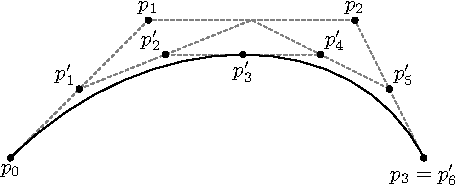
\includegraphics{subdivision}
% 	     \caption{A Figure}
% 	 \label{subd}
% 	\end{figure}

% \clearpage %% starts a new page and stops trying to place floats such as tables and figures

% \section{More Figure Stuff}
% You can also scale and rotate figures.
%  	\begin{figure}[h!]
	   
% 	       \centering
% 	    % DO NOT ADD A FILENAME EXTENSION TO THE GRAPHIC FILE
% 	    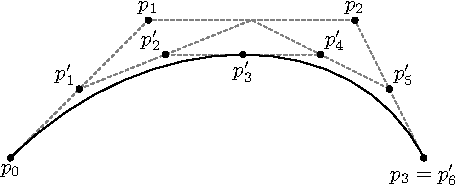
\includegraphics[scale=0.5,angle=180]{subdivision}
% 	    % if your figure shows up not where you want it, it may just be too big to fit. You can use the scale argument to shrink it, e.g. scale=0.85 is 85 percent of the original size. 
% 	     \caption{A Smaller Figure, Flipped Upside Down}
% 	 \label{subd2}
% 	\end{figure}

% \section{Even More Figure Stuff}
% With some clever work you can crop a figure, which is handy if (for instance) your EPS or PDF is a little graphic on a whole sheet of paper. The viewport arguments are the lower-left and upper-right coordinates for the area you want to crop.

%  	\begin{figure}[h!]
% 	    	       \centering
% 	    % DO NOT ADD A FILENAME EXTENSION TO THE GRAPHIC FILE
% 	   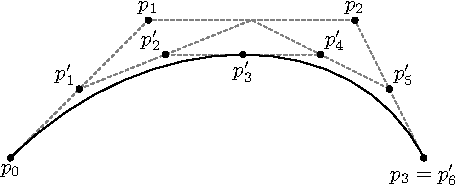
\includegraphics[clip=true, viewport=.0in .0in 1in 1in]{subdivision}
% 	    \caption{A Cropped Figure}
% 	 \label{subd3}
% 	\end{figure}
	
%       \subsection{Common Modifications}
   %    The following figure features the more popular changes thesis students want to their figures. This information is also on the web at \url{web.reed.edu/cis/help/latex/graphics.html}.
   %  %\renewcommand{\thefigure}{0.\arabic{figure}} 	% Renumbers the figure to the type 0.x
   %  %\addtocounter{figure}{4} 						% starts the figure numbering at 4
   %  \begin{figure}[htbp]
   %  \begin{center}
   % 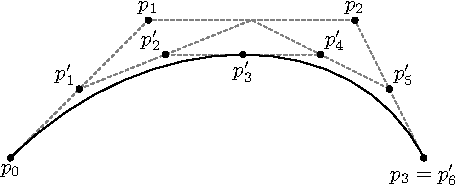
\includegraphics[scale=0.5]{subdivision}
   %  \caption[Subdivision of arc segments]{\footnotesize{Subdivision of arc segments. You can see that $ p_3 = p_6^\prime$.}} %the special ToC caption is in square brackets. The \footnotesize makes the figure caption smaller
   %  \label{barplot}
   %  \end{center}
   %  \end{figure} 

% \chapter*{Conclusion}
%          \addcontentsline{toc}{chapter}{Conclusion}
% 	\chaptermark{Conclusion}
% 	\markboth{Conclusion}{Conclusion}
% 	\setcounter{chapter}{4}
% 	\setcounter{section}{0}
	
% Here's a conclusion, demonstrating the use of all that manual incrementing and table of contents adding that has to happen if you use the starred form of the chapter command. The deal is, the chapter command in \LaTeX\ does a lot of things: it increments the chapter counter, it resets the section counter to zero, it puts the name of the chapter into the table of contents and the running headers, and probably some other stuff. 

% So, if you remove all that stuff because you don't like it to say ``Chapter 4: Conclusion'', then you have to manually add all the things \LaTeX\ would normally do for you. Maybe someday we'll write a new chapter macro that doesn't add ``Chapter X'' to the beginning of every chapter title.

% \section{More info}
% And here's some other random info: the first paragraph after a chapter title or section head \emph{shouldn't be} indented, because indents are to tell the reader that you're starting a new paragraph. Since that's obvious after a chapter or section title, proper typesetting doesn't add an indent there. 


%If you feel it necessary to include an appendix, it goes here.
%This is where endnotes are supposed to go, if you have them.
%I have no idea how endnotes work with LaTeX.

  \backmatter % backmatter makes the index and bibliography appear properly in the t.o.c...

% if you're using bibtex, the next line forces every entry in the bibtex file to be included
% in your bibliography, regardless of whether or not you've cited it in the thesis.

% Rename my bibliography to be called "Works Cited" and not "References" or ``Bibliography''
\renewcommand{\bibname}{References}

%    \bibliographystyle{bsts/mla-good} % there are a variety of styles available; 
%  \bibliographystyle{plainnat}
% replace ``plainnat'' with the style of choice. You can refer to files in the bsts or APA 
% subfolder, e.g. 
\singlespacing
\bibliography{thesis}
\bibliographystyle{apa}  % or
\nocite{*}

 % Comment the above two lines and uncomment the next line to use biblatex-chicago.
 %\printbibliography[heading=bibintoc]

% Finally, an index would go here... but it is also optional.
\end{document}
